\clearpage{}
\section{Describe and compare different strategies for integration testing,
and the need for stubs and drivers. Discuss the case of testing
object-oriented designs. Cite software tools that can be used for program
testing and analysis. Describe fault estimation using fault seeding and by
independent test groups.}

\subsection{Drivers and stubs}

How can you test a function that depends on other functions? \newline
Use test drivers and stubs.

\begin{description}
    \item[Driver] a program that calls a component (passes a test case to it).
    \item[Stub] a program that is called by a component (simulates the activity of a missing component), i.e.\ function which simulates the behaviour of the called function\ldots
\end{description}

\textbf{Never modify a component to support testing!} Drivers and stubs are separate programs.

\subsection{Strategies for integration testing}

\begin{figure}[!ht]
    \centering
    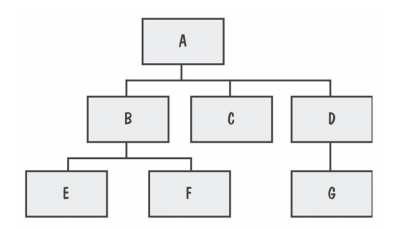
\includegraphics[width=0.5\linewidth]{strategies_integration_testing.png}
\end{figure}
Consider the component hierarchy

\subsubsection{Bottom-up}

Useful if many general-purpose utility routines, reused components at lowest level. \newline
Needs drivers.

\begin{figure}[!ht]
    \centering
    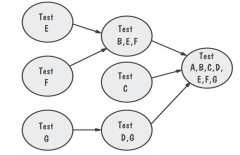
\includegraphics{bottom_up.png}
\end{figure}


\begin{itemize}
    \item[+] Suitable for object-oriented programs
    \item[-] The top-level components are tested last (most important, may reveal design bugs)
\end{itemize}

\subsubsection{Top-down}
Test the top-level, controlling component first.
Needs stubs.

\begin{figure}[!ht]
    \centering
    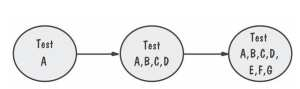
\includegraphics{top_down.png}
\end{figure}

\begin{itemize}
    \item[+] Allows test by external function
    \item[+] Major design faults or issues revealed early
    \item[+] Drivers not needed
    \item[-] Stubs can be difficult to develop, affects validity of the test
\end{itemize}

\subsubsection{Modified top-down}
Test components individually before integrating components

\begin{figure}[!ht]
    \centering
    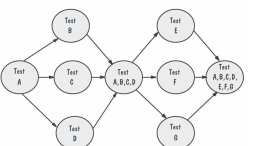
\includegraphics{modified_top_down.png}
\end{figure}

\begin{itemize}
    \item[+] Avoids large number of stubs
    \item[-] Needs stubs and drivers
\end{itemize}

\subsubsection{Bing-bang}
Everything integrated in one shot.
For small systems only.

\begin{figure}[!ht]
    \centering
    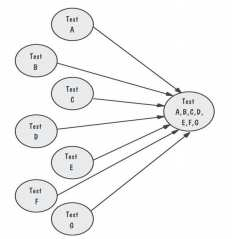
\includegraphics{bing_bang.png}
\end{figure}

\begin{itemize}
    \item[-] Needs drivers and stubs
    \item[-] Faults are hard to localize
    \item[-] Interface faults are hard to distinguish
\end{itemize}

\subsubsection{Sandwich}
Combine bottom-up and top-down, converge to target middle layer.

\begin{figure}[!ht]
    \centering
    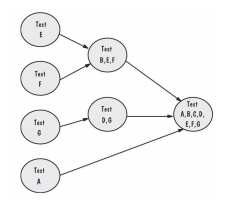
\includegraphics{sandwich.png}
\end{figure}

\begin{itemize}
    \item[+] Early test of top layer
    \item[-] No stubs for utility components in bottom layer
\end{itemize}

\subsubsection{Modified sandwich}
Test upper-level components before merging.

\begin{figure}[!ht]
    \centering
    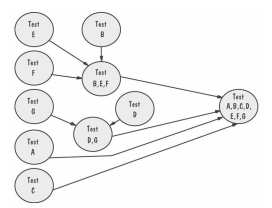
\includegraphics{modified_sandwich.png}
\end{figure}

\subsubsection{Comparison}

\begin{figure}[!ht]
    \centering
    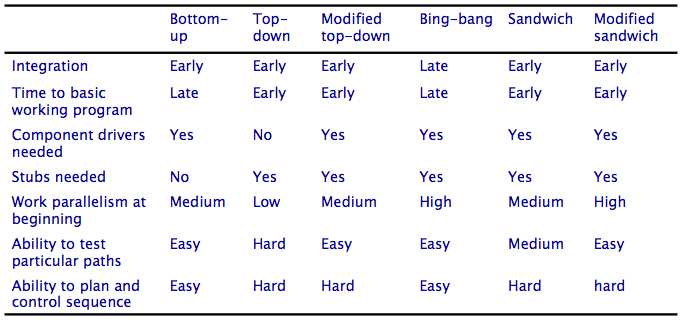
\includegraphics[width=\linewidth]{comparison_stategies_integration_testing.png}
\end{figure}

All except bottom-up need stubs!
All except top-down need drivers!

\subsection{Testing object-oriented designs}
Unit testing is easier but integration testing is more extensive. \newline

Ex: Dynamic binding, complex interface, polymorphism, inheritance are aspect related to OO which cause difficulties during test.

\subsection{Software tools for program testing and analysis}

\subsubsection{Automated testing tools}

Test execution: planning and running of the tests

\begin{itemize}
    \item Capture and replay (keystrokes)
    \item Generating stubs and drivers
    \item Automated testing environments (database, measurement, analysis, simulation,\ldots)
\end{itemize}

Test case generators:

\begin{itemize}
    \item Structural (structure of source code)
    \item Functional (specifications)
    \item Random
\end{itemize}

\subsubsection{Code analysis tools}

Static analysis: analyse the source code

\begin{itemize}
    \item Code analyser
    \item Structure checker
    \item Data analyser
    \item Sequence checker
    \item Measurements: paths, fan-in/fan-out, decision points,\ldots
    \item Program provers
\end{itemize}

Dynamic analysis: execute the program

\begin{itemize}
    \item Program monitoring (coverage)
    \item Instrumentation, breakpoints
\end{itemize}

\subsection{Fault estimation}

How to estimate how many faults remain? (Help us to know how to stop tests) \newline

Intentionally insert faults in the program:

\begin{itemize}
    \item A known number $S$
    \item Same kind and complexity as actual faults
\end{itemize}

Use the number of discovered seeded faults s and the number of discovered actual faults $n$ to estimate the number of actual faults $N$.\newline

Hypothesis: same effectiveness $\rightarrow n / N = s / S \rightarrow N = S \times n / s$

\todo[inline]{Manque Independent test groups<w}
